\section*{Chapter 1}
\begin{thmpf}{sqrt2irr}
    $\sqrt{2}$ cannot be written as a fraction.
    \tcblower
    We'll tackle this one by what's called \df{contradiction}: we'll assume it's not true, and prove that something impossible happens, so it must be true. 

    So, if it's not true, then $\sqrt{2}$ must be able to be written as a fraction. Let's call the numerator of that fraction $b$ and the denominator $c$, so that $\sqrt{2} = \dfrac{b}{c}$. There will be lots of ways to write $\sqrt{2}$ as a fraction (we also have $\sqrt{2} = \dfrac{2b}{2c} = \dfrac{3b}{3c} = \cdots$), so to make sure we don't cause any problems, we'll pick the one that makes $b$ (and so also $c$ as small as possible).

    But now, let's multiply both sides of that by $c$, so that $b = \sqrt{2}c$. Looking at that, I can see that $\sqrt{2}$ is the hardest part to think about, so we'll get rid of it by squaring both sides to get $b^2 = 2\times c^2$. 

    That tells us that $b^2$ is even: we just wrote it as 2 multiplied by a whole number. But that means that $b$ is even (because multiplying two odd numbers together gives an odd number). Since $b$ is even, we can write it as $2$ multiplied by a whole number. Let's say $b = 2\times d$, where $d$ is that whole number.

    But now we can replace $b$ with $2 \times d$ in the equation above, since they're the same, giving $(2 \times d)^2 = 2 \times c^2$. If we expand out those brackets, that gives us $4 \times d^2 = 2 \times c^2$, and we can divide both sides by $2$ to get $2 \times d^2 = c^2$. But just like before, that means that $c^2$ is even, so $c$ is even, so we can write $c = 2e$ with $e$ a whole number. 
    But then $\sqrt{2} = \dfrac{b}{c} = \dfrac{2d}{2e} = \dfrac{d}{e}$, but we just wrote $\sqrt{2}$ as a fraction with the numbers smaller than $b$ and $c$, which we said was impossible right at the start.

    Now we've found something impossible, our assumption at the start must be false, which is exactly what we were trying to prove. 
\end{thmpf}

We shall now work out the details of \ref{combrot} on page \pageref{combref}
\begin{proof}\label{combrotpf}
    
    We have this picture:
    \begin{tikzpicture}
        \coordinate (P) at (0,0);
        \coordinate (Q) at (2,1);
        \coordinate (R) at (-1.5,3);
        \coordinate (Pprime) at (4,2);
        \coordinate (Rprime) at (3.75,0);
        \coordinate (Qprime) at (1,-2);
        \node[anchor=east] at (0,0) {$p$};
        \filldraw (0,0) circle (2pt);
        \node[anchor=north] at (2,1) {$q$};
        \filldraw (2,1) circle (2pt);
        \draw[dashed] (-2,-1) -- (4,2);
        \node[anchor=south east] at (4,2) {$L$};
        \draw[dashed] (1,-2) -- (-2,4);
        \node[anchor=south west] at (-2,4) {$M$};
        \draw[dashed] (3.75,0) -- (-1.5,3);
        \node at (3.75,0) {$N$};
        \pic [draw, "$\frac{b}{2}$", angle eccentricity=1.5] {angle = R--Q--P};
        \pic [draw, "$\frac{a}{2}$", angle eccentricity=1.5] {angle = Qprime--P--Pprime};
    \end{tikzpicture}
    
     We've already shown that this is a rotation around the point where $M$ and $N$ cross by twice the angle between them. What actually need to do is work out where the lines cross and at what angle. 

    First, though, there's one slight issue: I've drawn my picture so that the lines cross above $L$, but they could just as easily cross below $L$, and this will change things slightly: we're now going to move our known angles inside the triangle, and one will end up staying the same, the other will be subtracted from $180\degree$, and which one gets changed will be different depending on where the lines cross. It won't end up making much difference though, so I'll just do the version I've drawn, and leave the other one up to you to try. 

    So, let's move the angle $\frac{a}{2}$ inside the triangle. If we just focus on that bit of the diagram, we've got two angles on a straight line where we know one of them is $\frac{a}{2}$, so the other must be $180\degree - \frac{a}{2}$. Then, we've got two of the three angles inside the triangles as $180\degree - \frac{a}{2}$ and $\frac{b}{2}$, so the third angle must be $180\degree - (180\degree - \frac{a}{2}) - \frac{b}{2} = \frac{a-b}{2}$. Notice that this is exactly the angle between the two lines we're reflecting in, so our rotation is by an angle of $a - b$ (if the lines crossed on the other side, we'd instead get $b - a$: notice that this happens exactly when $b > a$, so we just always get whichever of $a - b$ and $b - a$ is positive: we'll call this $|a - b|$). 

    So now we know all three angles of our triangle, as well as one of the sides (we know where $p$ and $q$ are, so we know how long the line between them is - for now, we'll call that length $x$), so we should be able to figure out the other sides as well. We'll use a thing called the \df{sine rule} for this: see Theorem \ref{sinerule} for the details. 

    This tells us that, if we call the length of the line from $p$ to our new point $y$ and the length of the line from $q$ to our new point $z$, we have 

    $$y = \dfrac{x\sin\left(\dfrac{b}{2}\right)}{\sin\left(\dfrac{a-b}{2}\right)}$$

    and 

    $$z = \dfrac{x\sin\left(180\degree - \dfrac{a}{2}\right)}{\sin\left(\dfrac{a-b}{2}\right)}$$

We can simplify that last one slightly: $\sin(180\degree - \theta) = \sin(\theta)$ for any angle $\theta$, so we can drop the ``$180\degree -$'' part: 

    $$z = \dfrac{x\sin\left(\dfrac{a}{2}\right)}{\sin\left(\dfrac{a-b}{2}\right)}$$

Now, let's be a little more careful and work out exactly where $M$ and $N$ cross, which I'll call $r$: first, let's add a line from $r$ to $L$ at right angles. 

\begin{tikzpicture}
	\coordinate (P) at (0,0);
	\coordinate (Q) at (2,1);
	\coordinate (R) at (-1.5,3);
	\coordinate (Pprime) at (4,2);
	\coordinate (Rprime) at (3.75,0);
	\coordinate (Qprime) at (1,-2);
	\node[anchor=east] at (0,0) {$p$};
	\filldraw (0,0) circle (2pt);
	\node[anchor=north] at (2,1) {$q$};
	\filldraw (2,1) circle (2pt);
	\draw[dashed] (-2,-1) -- (4,2);
	\node[anchor=south east] at (4,2) {$L$};
	\draw[dashed] (1,-2) -- (-2,4);
	\node[anchor=south west] at (-2,4) {$M$};
	\draw[dashed] (3.75,0) -- (-1.5,3);
	\node at (3.75,0) {$N$};
	\pic [draw, "$\frac{b}{2}$", angle eccentricity=1.5] {angle = R--Q--P};
	\pic [draw, "$\frac{a}{2}$", angle eccentricity=1.5] {angle = Qprime--P--Pprime};
	\node[anchor=south west] at (-1.5,3) {$r$};
	\draw (-1.5,3) -- (0.25,0.1);
\end{tikzpicture}

This gives us two right-angled triangles, but we only really need one, so I'll pick the one with $q$ in it. In this triangle, we know that the angle at $q$ is $\frac{b}{2}$, and the length from $q$ to $r$ is $z$, so the length of the bit of $L$ that's part of this triangle is $z\cos\left(\frac{b}{2}\right)$ and the length of the other shorter side is $z\sin\left(\frac{b}{2}\right)$. 

That's actually everything we need to know to work out exactly where $r$ is: first, we can find where it is in the ``$L$'' dimension: it's at $$q - z\sin\left(\frac{b}{2}\right)\left(\dfrac{1}{x}(p - q)\right) = q - \dfrac{\sin\left(\dfrac{a}{2}\right)\sin\left(\dfrac{b}{2}\right)}{\sin\left(\dfrac{a-b}{2}\right)}(p-q),$$ and secondly, we can find how far away from $L$ it is: it's $z\sin\left(\frac{b}{2}\right)$ away. 

Now, let's just abbreviate some things: let's define $\mathrm{Par}(a,b) = \dfrac{\sin\left(\dfrac{a}{2}\right)\cos\left(\dfrac{b}{2}\right)}{\sin\left(\dfrac{a-b}{2}\right)}$ and $\mathrm{Per}(a,b) = \dfrac{\sin\left(\dfrac{a}{2}\right)\sin\left(\dfrac{b}{2}\right)}{\sin\left(\dfrac{a-b}{2}\right)}$. I'm also going to define, for any vector $v = (g,h)$, $v^\perp := (-h,g)$ (the funny upside-down T thing is a ``perpendicular'' sign - feel free to check that the line from $(0,0)$ to $v^\perp$ is actually at right angles to the line from $(0,0)$ to $v$, which is where the name comes from). 

This then makes our formulas look nicer: we now know that $r = q - \mathrm{Par}(a,b)(p - q) + \mathrm{Per}(a,b)(p - q)^\perp$ (if the crossing is on the other side, you'll get a $-$ sign where I have a $+$), but since $\sin(-x) = -\sin(x)$, that's just the same as swapping whether we're using $a - b$ or $b - a$.  
\end{proof}


\begin{thmpf}{transcomb}
    Take any point: say it's $(a,b)$. Then our first translation moves it to $(a+x,b+y)$, and the second moves that to $(a+x+z,b+y+w)$, which is exactly where translating by $x+z$ horizontally and $y+w$ vertically would move it to. Since that works for every point, they must be the same. 
\end{thmpf}

\begin{theorem}
    Rotating by an angle $a$ around a point $p$ then translating by $v = (x,y)$ is the same as rotating by $a$ around $q$, where $q$ is the point at a distance of $\frac{|v|}{\sin(a)}$ from $p$ at an angle of $a$ from $v$.
\end{theorem}
\begin{proof}\label{rottranspos}
    Everything except the calculation of $q$ is given on page \ref{rottrans}. To find $q$, we'll draw a picture:
    
    \begin{tikzpicture}
        \node[anchor = north east] at (0,0) {$p$};
        \draw [very thick,->] (0,0) -- (3,2);
        \node[anchor = south east] at (1.5,1) {$v$};
        \node[anchor = north east] at (39/7,-13/7) {$q$};
        \draw (-2,3) -- (4,-6);
        \draw (2.333,3) -- (8.333,-6);
        \draw (-3,1) -- (9,-3);
        \coordinate (P) at (0,0);
        \coordinate (Q) at (39/7,-13/7);
        \coordinate (R) at (3,2);
        \pic [draw, "$a$", angle eccentricity=1.5] {angle = Q--P--R};
    \end{tikzpicture}
    
    Since the two parallel mirror lines are both at right angles to $v$, we have a right-angled triangle. Applying the definition of cosine gives the result. 
\end{proof}



\begin{invsol}{transrot}
    Write the translation as two reflections in lines perpendicular to $v$, with the first $-v$ away from $p$, the second through $p$. Write the rotation as two reflections through $p$, with the first perpendicular to $v$, the second at an angle of $a/2$ to the first. The two reflections through $p$ perpendicular to $v$ cancel, leaving two reflections in lines at an angle of $a/2$ to each other, which give a rotation by $a$. 

    To find the point we rotate around, let's draw a picture: 
    
    \begin{tikzpicture}
        \draw (0,1) -- (0,-6);
        \draw[very thick,->] (0,0) -- (3.1,0); 
        \draw (4,4/3) -- (-1,-20/3);
        \node[anchor = south] at (1.5,0) {$v$};
        \node[anchor = north west] at (3.1,0) {$p$};
        \node[anchor = north west] at (0,-5) {$q$};
        \coordinate (P) at (3.1,0);
        \coordinate (Q) at (0,0);
        \coordinate (R) at (0,-5);
        \pic [draw, "$a$", angle eccentricity=1.5] {angle = P--R--Q};
    \end{tikzpicture}

    This is a right-angled triangle, so the length from $p$ to $q$ is $\frac{|v|}{\sin(a)}$, and the angle from $p$ to $q$ is $a + 180\degree$, which tells us exactly where $q$ is. 
\end{invsol}

\begin{theoremwname}{The Sine Rule}\label{sinerule}
	For any triangle with angles $a$, $b$, and $c$ opposite sides of length $A$, $B$, and $C$, we have \[\dfrac{\sin(a)}{A} = \dfrac{\sin(b)}{B} = \dfrac{\sin(c)}{C}.\]
\end{theoremwname}
\begin{proof}
	Let's draw a picture:
	
	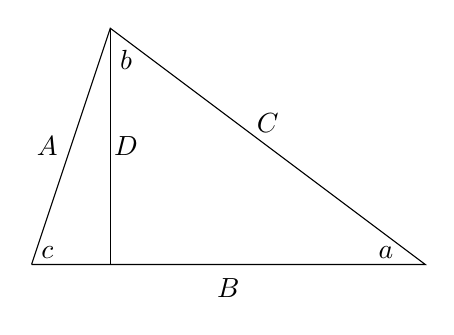
\begin{tikzpicture}
		\draw (0,0) -- (5,0) -- (1,3) -- (0,0);
		\draw (1,3) -- (1,0);
		\node at (0.2,1.5) {$A$};
		\node at (2.5,-0.3) {$B$};
		\node at (3,1.8) {$C$};
		\node at (4.5,0.15) {$a$};
		\node at (1.2,2.6) {$b$};
		\node at (0.2,0.15) {$c$};
		\node at (1.2,1.5) {$D$};
	\end{tikzpicture}
	
	You'll notice that we've added a line splitting our triangle into two right-angled triangles. Now, let's use the definition of sine in the right-hand triangle: that gives us \[\sin(a) = \dfrac{D}{C}.\] Doing the same on the left-hand triangle gives us \[\sin(c) = \dfrac{D}{A}.\] Rearranging those two gives $C\sin(a) = D = A\sin(c)$, and rearranging those gives us \[\dfrac{\sin(a)}{A} = \dfrac{\sin(c)}{C}.\] The same argument with the triangle rotated will give \[\dfrac{\sin(b)}{B} = \dfrac{\sin(a)}{A},\] so we're done.
\end{proof}